%=========================================================================
% sec-opts-copy
%=========================================================================

\section{Copying Blocks to Scratchpad}
\label{sec-opts-copy}

% Reason for optimization
\subsection{Reason for Optimization}

Although the blocking optimization helps the working set of a single
iteration of the computation kernel fit in the cache, it does not prevent
conflict misses in the cache. This is because blocking only reduces the
number of cache lines touched by the computation kernel, but does not
change the stride of the memory access pattern when traversing the columns
of a matrix. If the number of cache lines in a column is roughly a
multiple of the number of sets in the cache, consecutive rows in the
matrix will map to the same set. This means that if we traverse the
columns of a matrix, we will only be able to use one set of the cache,
causing repeated conflict misses. To makes things worse, only one element
of each new cache line we bring in will be used by the computation
kernel, yielding an inefficient utilization of the cache.
\smallskip

For example, the Intel Xeon processors on the totient compute nodes
have an 8-way set-associative L1 cache with a capacity of 32KB and 64B
lines. This means we have a total of $32K/64 = 512$ cache lines spread
out across $512/8 = 64$ sets. Assuming the matrix is arranged in
column-major order and in contiguous memory, the worst case is if the
matrix dimension is a multiple of $64*8 = 512$ doubles (since each cache
line can hold eight 64b doubles). Of course this only accounts for a
single matrix being stored in the cache--in reality, cache conflicts can
be aggravated with cache lines from multiple matrices being mapped to the
same set.
\smallskip

% Details of optimization
\subsection{Details of Optimization}

%=========================================================================
% fig-opts-copy-ex.tex
%=========================================================================

\begin{figure}[b]

  \centering
  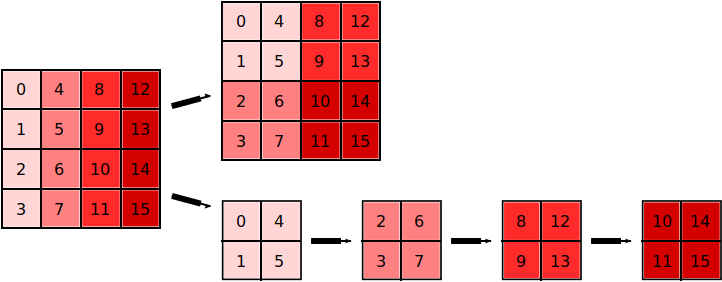
\includegraphics[width=0.9\tw]{fig-opts-copy-ex.svg.pdf}

  \caption{\textbf{Two Approaches to Copy Optimization --} The matrix on
    the left is arranged in column-major order in memory. It can be
    copied into a large scratchpad capable of storing all blocks (top
    path), or copied into a smaller scratchpad with enough space for one
    block (bottom path). In either case the data in each block is
    arranged to be contiguous in memory. The indices represent the data
    element in the original matrix and the colors represent contiguous
    segments in memory, with darker colors representing increasing
    addresses in memory.}

  \label{fig-opts-copy-ex}

\end{figure}


We can alleviate such conflicts and reduce the sensitivity to matrix
dimensions by copying blocks into a scratchpad such that the data within
each block are contiguous in memory. This allows us to control the stride
of traversing the columns within a block regardless of the matrix
dimensions by setting the block dimensions such that these conflicts
become rare. Furthermore, if we set the block dimensions such that all
matrices fit in the L1 cache, we can get closer to fully utilizing the
cache capacity without any conflicts. In addition, this copy optimization
allows us to align the matrices to the SIMD width regardless of the
matrix dimensions to enable vector loads/stores when vectorizing the
code. A critical tradeoff to keep in mind is the computational cost of
copying the matrices to the scratchpad memory. This optimization only
makes sense if the benefit of reducing conflict misses in the cache
outweighs the overhead of the copy itself.
\smallskip

Figure~\ref{fig-opts-copy-ex} shows how an example 4x4 matrix using 2x2
blocks are re-arranged when copying to the scratchpad memory. There are a
couple approaches to when and how much data to copy. One approach is to
copy and re-arrange the entire matrix once before any computation, then
copy the result back from the scratchpad to the output matrix in the
original format after the computation is complete. This amortizes the
overhead of bringing in the data from the input matrices into the cache
over the entire computation, but it increases memory pressure by
requiring a scratchpad that can hold all three matrices. Another approach
is to only allocate enough space in the scratchpad for three blocks and
copy the data in and out of the scratchpad every iteration of the
computation kernel. This makes more efficient use of memory, but we need
to contaminate the cache with data from the original input matrices
between every call to the computation kernel.
\smallskip

% Results and analysis
\subsection{Results}

%=========================================================================
% fig-opts-copy-results.tex
%=========================================================================

\begin{figure}[b]

  \centering
  \includegraphics[width=0.7\tw]{fig-opts-copy-results.pdf}

  \caption{\textbf{Performance Comparison of Copy Optimizations --}
    We show results for a large scratchpad with a single copy of the
    entire matrix before/after the computation, and a small scratchpad
    with multiple copies of just the blocks being used for the current
    iteration of the computation kernel. We intentionally omit the
    results for BLAS and MKL implementations in order to focus on the
    behavior at the performance range of the optimization.}

  \label{fig-opts-copy-results}

\end{figure}


Figure~\ref{fig-opts-copy-results} shows the results for both large and
small scratchpad approaches to copy optimization. The interesting point
here is although there are no performance improvements, the performance
is much more stable across all matrix dimensions. This emphasizes the
impact of conflict misses in the cache from the matrix dimensions.

A quick note on choosing block sizes. We theorize that the optimal block
size is one which allows all three blocks to fit completely inside of the
L1 cache. With a 32KB cache, the following equation must be satisfied:
\[
3M^2 <= \frac{32K}{8} \rightarrow M <= \sqrt{\frac{32K}{8*3}} \rightarrow M <= 37
\]
\smallskip

However, a sweep of the block sizes showed that a block size of 128 was
optimal across all matrix dimensions. This likely has to do with the fact
that the computation kernel requires more data from one block than the
other blocks at a given iteration, so it is preferable to have a larger
block size to better amortize the overhead of calling a computation
kernel iteration.

